\documentclass[conference]{IEEEtran}
\IEEEoverridecommandlockouts
% The preceding line is only needed to identify funding in the first footnote. If that is unneeded, please comment it out.
\usepackage{cite}
\usepackage{amsmath,amssymb,amsfonts}
\usepackage{algorithmic}
\usepackage{graphicx}
\usepackage{textcomp}
\usepackage{xcolor}
\usepackage{ctex}
\usepackage{fontspec}
\usepackage{listings}
\usepackage{pxfonts}
% The following code is for matlab language
\lstset{
    columns=fixed,     
    basicstyle = \tt,           % 基本样式 + 小号字体  
    %numbers=left,    % 在左侧显示行号
    frame=none,     % 不显示背景边框
    breaklines = true,                  % 代码过长则换行
    backgroundcolor=\color[RGB]{245,245,244},  % 设定背景颜色
    keywordstyle=\color[RGB]{40,40,255},         % 设定关键字颜色
    % numberstyle=\footnotesize\color{darkgray},    % 设定行号格式
    commentstyle=\it\color[RGB]{0,96,96},         % 设置代码注释的格式
    stringstyle=\rmfamily\slshape\color[RGB]{128,0,0},   % 设置字符串格式
    showstringspaces=false,   % 不显示字符串中的空格
    language=python,             % 设置语言
    extendedchars=false,
    %basicstyle=Consolas
    tabsize=4,
    upquote=true,
    %literate={'}{\textquotedb}1
    morekeywords={as,convolve,&,sinc, plot, xlim,ylim,title,fontsize,np,subplot,show,subplots_adjust, suptitle},
}

\def\BibTeX{{\rm B\kern-.05em{\sc i\kern-.025em b}\kern-.08em
    T\kern-.1667em\lower.7ex\hbox{E}\kern-.125emX}}
\begin{document}

\title{傅立叶变换光谱测量技术实验报告}

\author{
    \IEEEauthorblockN{
        黄润华}
        \IEEEauthorblockA{
            \textit{Ocean University of China} \\
            \textit{email@noreply.com}
    \and
    \IEEEauthorblockN{
        杨超}
        \IEEEauthorblockA{
            \textit{Ocean University of China} \\
            \textit{email@somewhere.com}
        }
    }
}

\maketitle

\begin{abstract}
本实验报告为傅立叶变换光谱测量技术第二次实验报告,本报告采用Python仿真同时考虑有限扫描长度和被测入射光发散角两因素影响下的傅里叶变换光谱测量系统的光谱测量曲线。
\end{abstract}

\begin{IEEEkeywords}
Optical spectrum, Python 
\end{IEEEkeywords}

\section{实验目的}
\begin{itemize}
\item 思考有限扫描长度对光谱测量的影响;
\item 思考被测入射光发散角对光谱测量的影响;
\item 学习利用Python仿真不同影响条件下光谱测量曲线。
\end{itemize}

\section{实验原理}
光谱仪的光谱分辨率是其定性区分彼此非常接近的两个光谱峰的能力的量度。 通常,光谱 分辨率由仪器线形状(ILS)的半峰全宽(FWHM)表示,光谱仪的输出光谱具有纯单色输入辐射。

光谱分辨率R由下式定义
\begin{align}
    R = \frac{\sigma_{max}}{\delta \sigma} \label{eq1}
\end{align} 
其中,$\sigma_{max}$是光谱仪设计运行的最大波数。

\subsection{分辨率与最大OPD之间的关系}
根据公式
\begin{align}
    B_{c}(\sigma)=B_{r e L}(\sigma)+i B_{i o L}(\sigma)=\int_{-\infty}^{\infty} I(x) \operatorname{rect}(x) e^{-i 2 \pi a x} d x \\
    \begin{cases}{c}
        B(\sigma)=2 \mid \int_{-\infty}^{+\infty} I(x) \operatorname{rect}(x) e^{-2 \pi a x} d x \\
        \phi(\sigma)=\arctan \left[\frac{B_{i o L}(\sigma)}{B_{r e L}(\sigma)}\right]
    \end{cases} \quad(\sigma \geq 0)
\end{align}
其中矩形函数定义为
\begin{align*}
    \operatorname{rect}(x)=\begin{cases}
        1 & |x|<L \\
        0 & |x|>L
        \end{cases}
\end{align*}
因此,理论上 FTS 的光谱分辨率取决于可移动镜的扫描范围
\begin{align}
    B_{e}(\sigma)=\begin{cases}{ll}
        B(\sigma) / 2 & (\sigma \geq 0) \\
        B(-\sigma) / 2 & (\sigma \leq 0)
        \end{cases}
\end{align}
理论上,完美单色线的干涉图可以用来描述
\begin{align}
    I(x) = 2cos(2\pi \sigma_0 x)
\end{align}
将此表达式替换为方程$B(\sigma)$、$\phi(\sigma)$,考虑到实际上$\sigma > 0$,可以得到ILS $B(\sigma)$的表达式:
\begin{align}
        B_{I I S}(\sigma)
        &=2 L\frac{\sin \left[2 \pi\left(\sigma_{0}+\sigma\right) L\right]}{2 \pi\left(\sigma_{0}+\sigma\right) L}+\frac{\sin \left[2 \pi\left(\sigma_{0}-\sigma\right) L\right]}{2 \pi\left(\sigma_{0}-\sigma\right) L} \\
        & \approx 2 L \times \frac{\sin \left[2 \pi\left(\sigma_{0}-\sigma\right) L\right]}{2 \pi\left(\sigma_{0}-\sigma\right) L}  \\
        & =2 L \sin c\left[2 \pi\left(\sigma_{0}-\sigma\right) L\right]
\end{align}
如图\ref{pic1}所示,光谱从一条线($\delta$ 函数)扩展到 $sin c$ 函数形状(仪器线形)。
\begin{align}
    (\delta \sigma)_{linewidth} = \frac{1.21}{2L}
\end{align}

\begin{figure}[htbp]
    \centerline{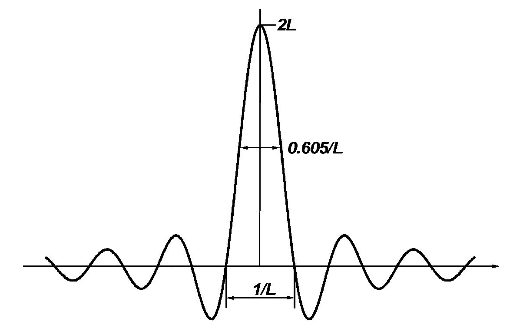
\includegraphics[width=0.5\textwidth]{pic1.png}}
    \caption{$B_{I I S}(\sigma)$}
    \label{pic1}
\end{figure}

\subsubsection{分离共振}
分辨率可以通过分离图\ref{pic2}所示光谱中相同强度(或共振)的两条单色线(波数和)来描述。
如果两个线峰值之间的下降幅度大于线峰值的 20\%,则可以声称解决了两个共振,此时
\begin{align}
    (\delta \sigma)_{separation} = \frac{1.46}{2L}
\end{align}

\begin{figure}[htbp]
    \centerline{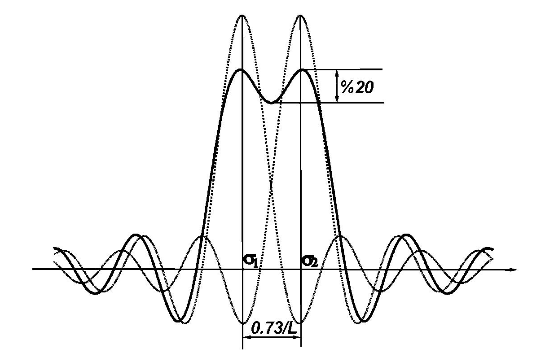
\includegraphics[width=0.5\textwidth]{pic2.png}}
    \caption{分离共振解析结果}
    \label{pic2}
\end{figure}

\subsubsection{瑞利准则}
瑞利准则分离两个 ILS 的峰值,使得一个共振的最大值落在另一个共振的零点处,因此,仪器线形状决定的分辨率是
\begin{align}
    \delta \sigma = \frac{1}{2L}    \label{eq2}
\end{align} 

\subsection{分辨率与发散角度之间的关系}
图\ref{pic3}是迈克尔逊干涉仪的等效图,根据图\ref{pic3}与图\ref{pic4}可以计算出OPD与夹角$\theta$之间的关系
\begin{align}
    O P D=2 \times \frac{x / 2}{\cos \theta}-x \tan \theta \sin \theta=x \cos \theta
\end{align}

\begin{figure}[htbp]
    \centerline{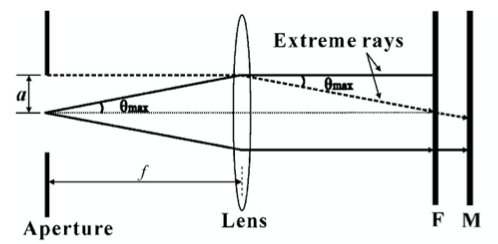
\includegraphics[width=0.5\textwidth]{pic3.png}}
    \caption{迈克尔逊干涉仪的等效图}
    \label{pic3}
\end{figure}

\begin{figure}[htbp]
    \centerline{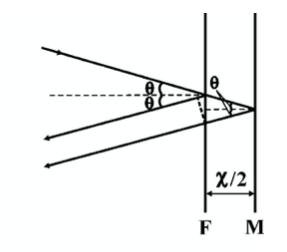
\includegraphics[width=0.5\textwidth]{pic4.png}}
    \caption{迈克尔逊干涉仪接收端放大图}
    \label{pic4}
\end{figure}
我们可以得到扩展源的归一化干涉图,对着一个立体角$\Omega_{max}$是
\begin{align*}
    I\left(x, \Omega_{\max }\right)=\frac{1}{\Omega_{\max }}\int_{0}^{\infty} B(\sigma) \int_{0}^{\Omega_{\operatorname{mix}}} \cos (2 \pi \sigma x \cos \theta) d \Omega d \sigma
\end{align*}
根据立体角的公式,上述式子可以化简为
\begin{align*}
    I\left(x, \Omega_{\max }\right)=\int_{0}^{\infty} B(\sigma) sinc \frac{\Omega_{\max } \sigma x }{2}  &\cos [2 \pi \sigma x\\
    & \;\;\;\;\;\;\;\;\;- \frac{\Omega_{\max } \sigma x }{2}] d \sigma
\end{align*}
对于单色光源其满足
\begin{align*}
    B(\sigma) = \delta(\sigma-\sigma_0)
\end{align*}
其仪器线轮廓可以写为
\begin{align*}
    \begin{cases}
        B_{D i v-1 L S}(\sigma)=[\pi /(\sigma_{0} \Omega_{\max })] \operatorname{rect}(\sigma_{1}, \sigma_{2})\\ \;\;\;\;\;\;\;\;\;\;\;\;\;\;\;\;\;\;\;\;\;\;\;\;\;\;\;\;\;\;\;\;+[\pi /(\sigma_{0} \Omega_{\max })] \operatorname{rect}(-\sigma_{2},-\sigma_{1}) \\
        \sigma_{2}=\sigma_{0}-\sigma_{0} \Omega_{\max } / 2 \pi \\
        \sigma_{1}=\sigma_{0}
    \end{cases}
\end{align*}
于是可以得到
\begin{align}
    &B_{D i v-1 L S}(\sigma)=\left[\pi /\left(\sigma_{0} \Omega_{\max }\right) \operatorname{lrect}\left(\sigma_{1}, \sigma_{2}\right)\right. \\
    &\bar{\sigma}=\sigma_{0}\left[1-\left(\Omega_{\max } / 4 \pi\right)\right]
\end{align}
总的波数差或分辨率是
\begin{align*}
    \delta \sigma = \frac{\sigma_0\Omega_{max}}{2\pi}
\end{align*}
考虑到可移动镜的扫描长度有限,实际 FTS 的 ILS 应该是
\begin{align}
    B_{I L S}(\sigma)=B_{D i v-I L S}(\sigma) * 2 L \sin c[2 \pi \sigma L]
\end{align}
其中$L$是可移动镜的最大位移,$*$是卷积算子。
图\ref{pic4}中两个极端射线的OPD之间的差异公式如下:
\begin{align*}
    \Delta O P D=2 L-2 L \cos \theta_{\max } \approx L \theta_{\max }^{2}=L \frac{a^{2}}{ f^{2}}
\end{align*}
其中$a$是入口孔径的半径,$f$是准直器的焦距。当$\Delta OPD$等于$\lambda/2$时,两条光线异相,它们之
间会发生破坏性叠加。对于宽带辐射输入,存在的最短波长决定了 FTS 的$\Delta OPD$的最大有效值, 如下式所示:
\begin{align}
    \Delta OPD \leq \frac{\lambda_{min}}{2} = \frac{1}{2\sigma_{max}}
\end{align}
结合上述两个方程式、式(\ref{eq1})和方程(\ref{eq2}),我们可以得到 $a$的值应满足以下不等式, 以获得大于$R$的分辨率:
\begin{align}
    a \leq \frac{f}{\sqrt{R}}
\end{align}

\section{实验内容}
仿真同时考虑有限扫描长度和被测入射光发散角两因素影响下的傅里叶变换光谱测量系统的光谱测量曲线。以 $632. 8nmm$的 HeNe 激光和 $532nm$ 激光为例。光程差采样间隔选定 $632. 8nm/8$。

\section{实验结果}
图\ref{pic5}展示了有限扫描长度和被测入射光发散角两因素影响下波长为$632.8nm$的HeNe激光的光谱测量曲线。
\begin{figure}[htbp]
    \centerline{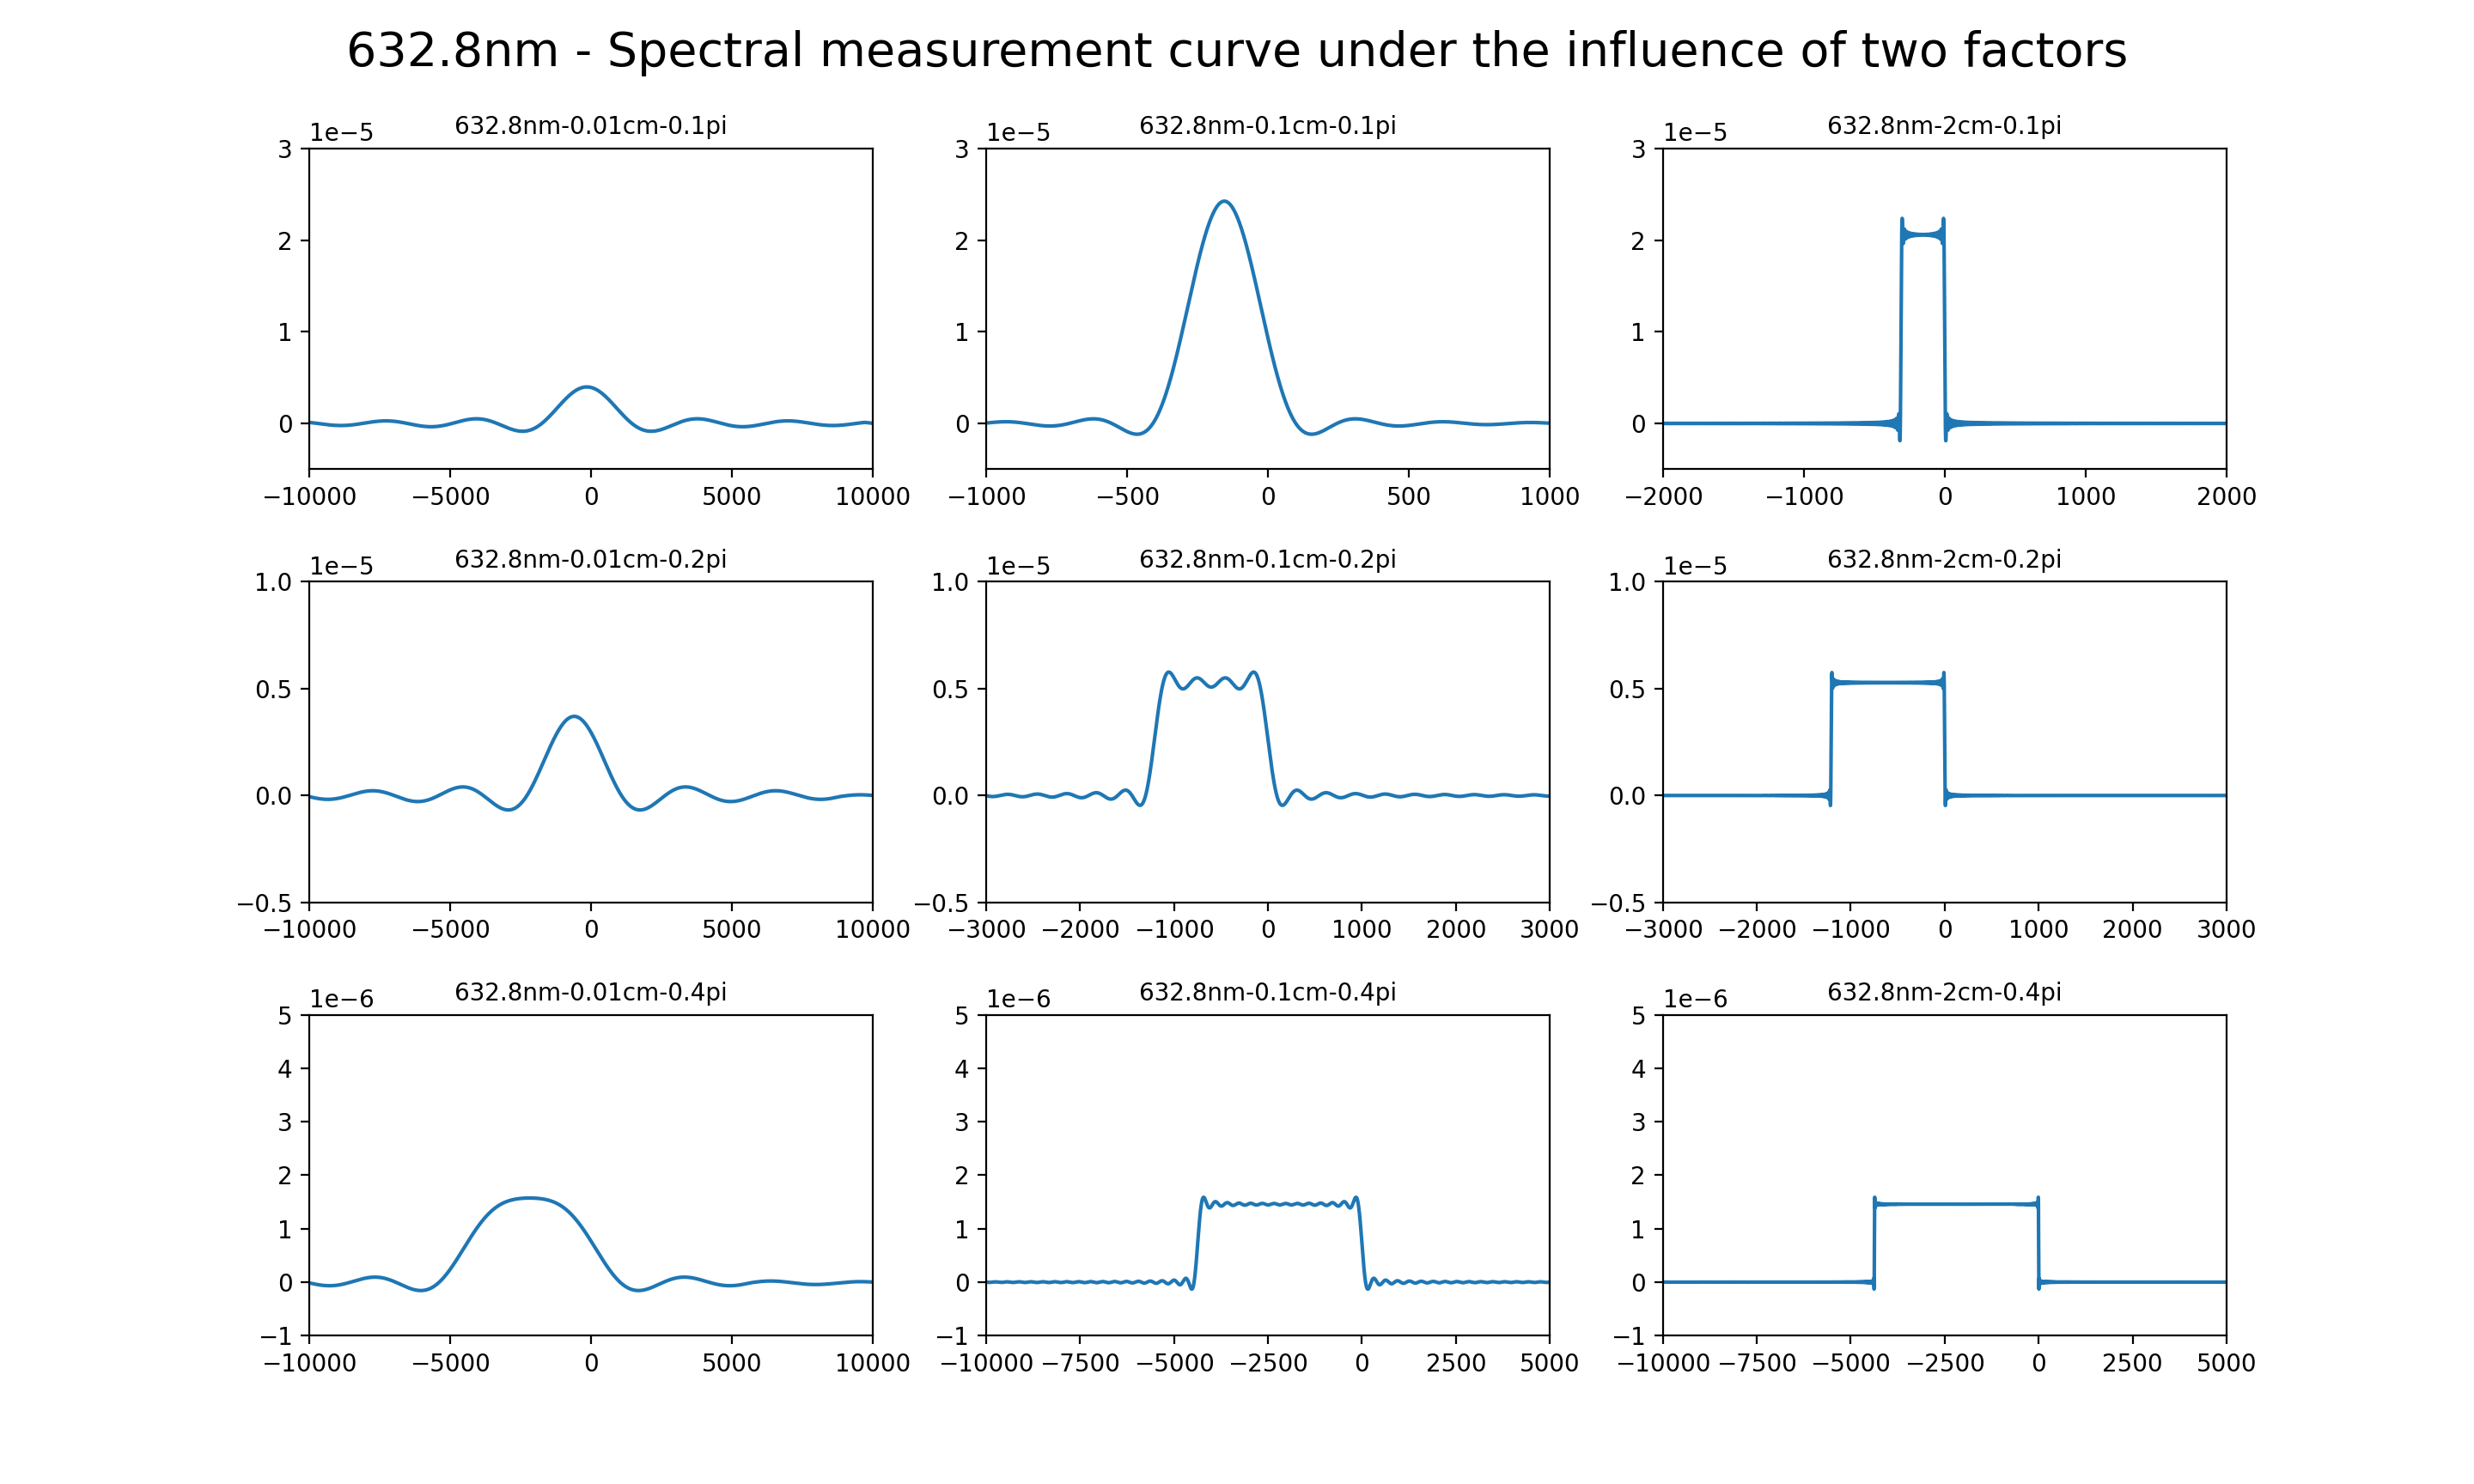
\includegraphics[width=0.5\textwidth]{pic5.png}}
    \caption{有限扫描长度和被测入射光发散角两因素影响下波长为$632.8nm$的HeNe激光的光谱测量曲线}
    \label{pic5}
\end{figure}
图\ref{pic6}展示了有限扫描长度和被测入射光发散角两因素影响下波长为$532nm$的激光的光谱测量曲线。
\begin{figure}[htbp]
    \centerline{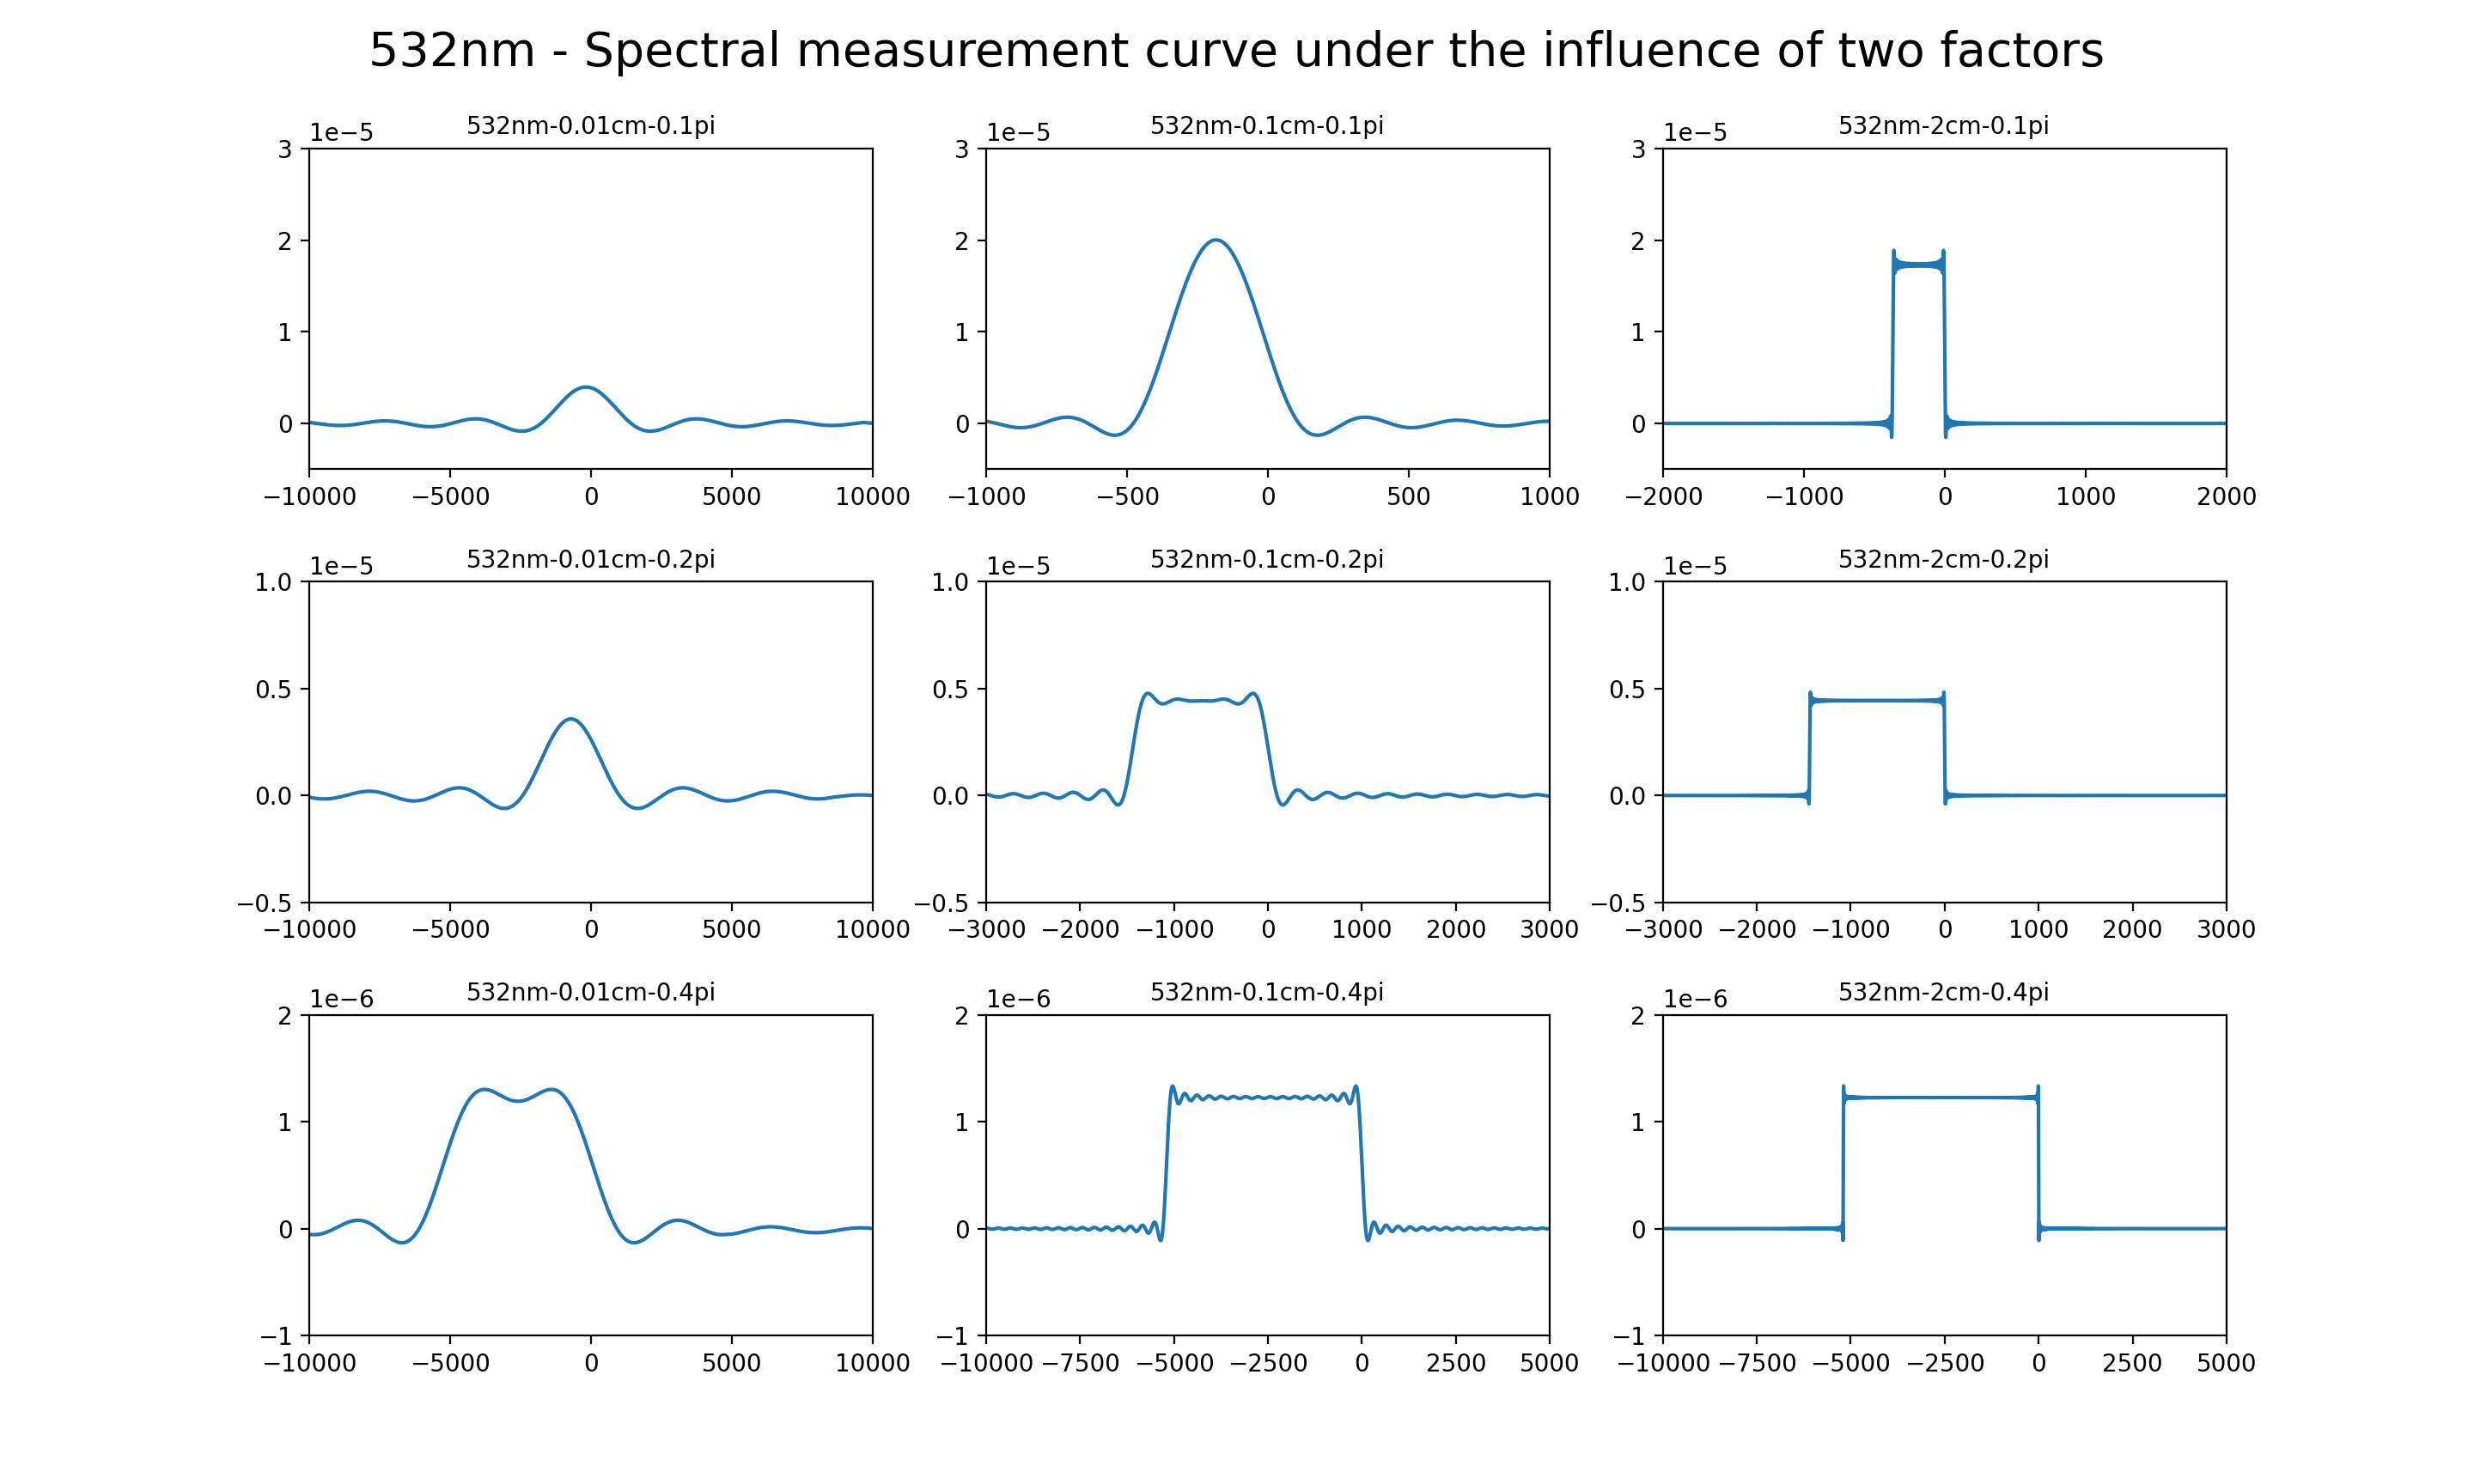
\includegraphics[width=0.5\textwidth]{pic6.png}}
    \caption{有限扫描长度和被测入射光发散角两因素影响下波长为$532nm$的激光的光谱测量曲线}
    \label{pic6}
\end{figure}
通过图\ref{pic5}与图\ref{pic6}可以得到如下结论:
\begin{itemize}
    \item 扫描长度越长,越集中,分辨率越高。
    \item 发散角度越大,宽度越大,幅度越小,分辨率越差。
    \item 两种影响同时存在时, 占主要地位的影响因素作用明显。
\end{itemize}

\section{结语}
本实验完成了利用Python仿真同时考虑有限扫描长度和被测入射光发散角两因素影响下的傅里叶变换光谱测量系统的光谱测量曲线的实验。




\appendix[实验代码(以波长为$632.8nm$的HeNe激光为例)]
\begin{lstlisting}
 import numpy as np
 import matplotlib.pyplot as plt
 from scipy.fftpack import fft, ifft
 from matplotlib.pylab import mpl
 from pylab import *
    
 # 设置扫描长度(m)
 L1 = 0.0001
 L2 = 0.001
 L3 = 0.02
    
 # 设置三个入射发散角
 sita1=0.1*np.pi 
 sita2=0.2*np.pi
 sita3=0.4*np.pi
    
 # 设置三个入射发散角的立体角
 W1=2*np.pi*(1-np.cos(sita1))
 W2=2*np.pi*(1-np.cos(sita2))
 W3=2*np.pi*(1-np.cos(sita3))
    
 # 设置波长
 L = 632.8*10**(-9)
    
 sigma0 = 1/L
 sigma1_1 = sigma0 - sigma0*W1/(50*np.pi)
 sigma1_2 = sigma0 - sigma0*W2/(50*np.pi)
 sigma1_3 = sigma0 - sigma0*W3/(50*np.pi)
 sigma2 = sigma0
    
 # 设置波束范围
 sigma = np.arange(sigma0 - 10**5, sigma2 + 10**5)
 sigma_jiehe = np.arange(-10**4, 10**4, 0.1)
    
 # 入射角的影响
 B1 = np.pi/(sigma0*W1)*((sigma>=sigma1_1)&(sigma<=sigma2))
 B2 = np.pi/(sigma0*W2)*((sigma>=sigma1_2)&(sigma<=sigma2))
 B3 = np.pi/(sigma0*W3)*((sigma>=sigma1_3)&(sigma<=sigma2))
    
 # 扫描长度的影响 
 Y01 = 2*L1*np.sinc(2*np.pi*sigma_jiehe*L1) 
 Y02 = 2*L2*np.sinc(2*np.pi*sigma_jiehe*L2) 
 Y03 = 2*L3*np.sinc(2*np.pi*sigma_jiehe*L3)
    
 # 卷积(长度和角度的影响)
 I1=np.convolve(B1,Y01,'same')
 I2=np.convolve(B1,Y02,'same')
 I3=np.convolve(B1,Y03,'same')
 I4=np.convolve(B2,Y01,'same')
 I5=np.convolve(B2,Y02,'same') 
 I6=np.convolve(B2,Y03,'same') 
 I7=np.convolve(B3,Y01,'same') 
 I8=np.convolve(B3,Y02,'same') 
 I9=np.convolve(B3,Y03,'same')
    
 plt.subplot(3,3,1)
 plt.plot(sigma_jiehe,I1)
 plt.xlim(-10000,10000)
 plt.ylim(-0.5*10**(-5),3*10**(-5))
 plt.title('632.8nm-0.01cm-0.1pi', fontsize = 10)
    
 plt.subplot(3,3,2)
 plt.plot(sigma_jiehe,I2)
 plt.xlim(-1000,1000)
 plt.ylim(-0.5*10**(-5),3*10**(-5))
 plt.title('632.8nm-0.1cm-0.1pi', fontsize = 10)
    
 plt.subplot(3,3,3)
 plt.plot(sigma_jiehe,I3)
 plt.xlim(-2000,2000)
 plt.ylim(-0.5*10**(-5),3*10**(-5))
 plt.title('632.8nm-2cm-0.1pi', fontsize = 10)
    
 plt.subplot(3,3,4)
 plt.plot(sigma_jiehe,I4)
 plt.xlim(-10000,10000)
 plt.ylim(-0.5*10**(-5),1*10**(-5))
 plt.title('632.8nm-0.01cm-0.2pi', fontsize = 10)
    
 plt.subplot(3,3,5)
 plt.plot(sigma_jiehe,I5)
 plt.xlim(-3000,3000)
 plt.ylim(-0.5*10**(-5),1*10**(-5))
 plt.title('632.8nm-0.1cm-0.2pi', fontsize = 10)
    
 plt.subplot(3,3,6)
 plt.plot(sigma_jiehe,I6)
 plt.xlim(-3000,3000)
 plt.ylim(-0.5*10**(-5),1*10**(-5))
 plt.title('632.8nm-2cm-0.2pi', fontsize = 10)
    
 plt.subplot(3,3,7)
 plt.plot(sigma_jiehe,I7)
 plt.xlim(-10000,10000)
 plt.ylim(-0.1*10**(-5),0.2*10**(-5))
 plt.title('632.8nm-0.01cm-0.4pi', fontsize = 10)
    
 plt.subplot(3,3,8)
 plt.plot(sigma_jiehe,I8)
 plt.xlim(-10000,5000)
 plt.ylim(-0.1*10**(-5),0.2*10**(-5))
 plt.title('632.8nm-0.1cm-0.4pi', fontsize = 10)
    
 plt.subplot(3,3,9)
 plt.plot(sigma_jiehe,I9)
 plt.xlim(-10000,5000)
 plt.ylim(-0.1*10**(-5),0.2*10**(-5))
 plt.title('632.8nm-2cm-0.4pi', fontsize = 10)
    
 plt.suptitle("632.8nm - Spectral measurement curve under the influence of two factors", fontsize = 20) 
    
 plt.subplots_adjust(left=0.125,
                     bottom=0.1, 
                     right=0.9, 
                     top=0.9, 
                     wspace=0.2, 
                     hspace=0.35)
 plt.show()
    
\end{lstlisting}

\end{document}
